\section{Casi d'uso}

\subsection{Attori}
\begin{figure}[h]

\caption{Gerarchia degli attori}
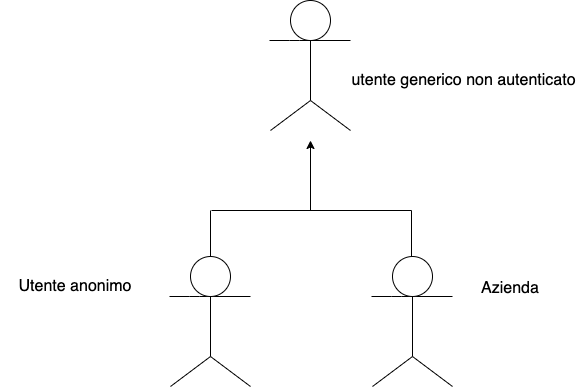
\includegraphics[width=7cm]{section/images/utenti.png}
\centering

\end{figure}
\begin{description}
\item[Utente generico]:
Si riferisce all'utente utilizzatore che può accedere alla piattaforma.
\item[Utente non autenticato]:
Riguarda l'utente che non possiede credenziali di accesso all'applicazione.
\item[Azienda] :
L'utente utilizzatore che accede alla piattaforma nel ruolo di azienda.
\end{description}
\subsection{Elenco casi d'uso}
In questa sezione vi sono elencati tutti i casi d'uso individuati. Ogni caso d'uso rappresenta uno scenario per uno o più attori.